% Notes:
% 
% 
\documentclass[rgb,dvipsnames]{beamer}
\usepackage[english]{babel}
\usepackage{xcolor}
\usepackage{listings}
\usepackage{adjustbox}
\newcommand{\LO}{$\mathcal{L}_0$}
\usepackage{amsmath}

\usepackage[linewidth=1pt]{mdframed}

% Graphics
\usepackage{graphicx}

% Font
\usepackage{paratype}
\setbeamerfont{frametitle}{family=\bf}


% Beamer theme settings
\usecolortheme{seagull}
\setbeamertemplate{itemize item}{\raisebox{0.8mm}{\rule{1.2mm}{1.2mm}}}
\usenavigationsymbolstemplate{} % no navigation buttons

\lstdefinelanguage{L0}
{keywords={fun,if,then,else,loop,do,map,reduce,filter,scan,redomap,mapT,reduceT,filterT,scanT,redomapT,transpose,reshape,iota,replicate,let,op,for,with},%
  sensitive=true,%
  comment=[l]{//},%
  string=[b]",%
  string=[b]'%
  basicstyle=\ttfamily\color{black},
  moredelim=**[is][\color{red}]{@}{@},
  moredelim=**[is][\color{blue}]{¤}{¤},
}

\lstset{
  language=L0
}

\title{Master's thesis defence}
\subtitle{Exploiting functional invariants to optimise parallelism:\\ A dataflow approach}
\author{Troels Henriksen (athas@sigkill.dk)}
\date{21. February 2014}
\institute{Computer Science\\
  University of Copenhagen}

\begin{document}

\frame{\titlepage}

\begin{frame}
  \frametitle{Part 0: Free lunches}

  \begin{columns}
    \begin{column}{0.3\textwidth}
      \small
      \color{OliveGreen} Transistors (thousands)

      \color{Blue} Clock Speed (MHz)

      \color{RoyalBlue} Power (W)

      \color{Purple} Perf/Clock (ILP)
    \end{column}
    \begin{column}{0.7\textwidth}
      \includegraphics[width=7cm]{img/CPU-Scaling.jpg}
    \end{column}
  \end{columns}

  \begin{itemize}
  \item Moore's law still in effect, and will be for a while...
  \item ... but we no longer get many increases in sequential
    performance.
  \end{itemize}

\end{frame}

\begin{frame}
  \frametitle{So, what's on the menu?}

  \begin{itemize}
  \item Modern performance increases are in the form of parallelism.
  \item The most parallel machines are massively parallel vector
    processors, with commodity GPUs particularly interesting due to
    being mainstream.
  \item GPUs were popularised in the 90s for graphics processing.
  \item Graphics is inherently parallel, so for cost reasons, the GPU
    hardware was very parallel as well.
  \item In roughly 2006, GPGPU began to take off with CUDA and then
    OpenCL.
  \end{itemize}
\end{frame}

\begin{frame}
  \frametitle{GPGPU programming}

  Three main ways to exploit GPGPU:

  \begin{description}
  \item[\bf Low-level interface:] Difficult to use,
    difficult to optimise.  Examples: OpenCL, CUDA.
  \item[\bf Libraries with optimised primitives:] Easy to use, but hard to
    optimise composition of primitives.  Example: GPU-implementations
    of BLAS.
  \item[\bf Specialised programming languages:] Can achieve good
    performance, yet still be easy to use.  Examples: NESL,
    Accelerate.
    \begin{itemize}
    \item Accelerate is very restricted - no nested parallelism.
    \item NESL compilation depends too much on flattening, which
      ignores communication overhead.
    \end{itemize}
  \end{description}
\end{frame}

\begin{frame}
  \frametitle{GPGPU programming, continued}

  What is needed in a high-level performance-oriented GPGPU language?

  \begin{description}
  \item[\bf Language features:] Performance guarantees from the language,
    particularly asymptotic ones.  Example: In-place updates.
  \item[\bf Language invariants:] Programs have properties that are always
    true-by-construction, and can be exploited to perform aggressive
    optimisation.  Example: Purely functional enabling loop fusion.
  \item[\bf Expressivity:] We need to be able to express interesting
    programs.  Example: Nested parallelism.
  \end{description}

  Existing languages are not sufficient: either they are too
  restricted (e.g. Accelerate), or not sufficiently optimised
  (e.g. NESL).  So we make our own: \LO{}.
\end{frame}

% \begin{frame}
%   \frametitle{Language design}

%   \begin{itemize}
%   \item Three real-world financial computational kernels served to
%     guide the design.  Two central questions:
%     \begin{itemize}
%     \item \textbf{What is the simplest language that permits a
%       relatively straightforward translation of the financial
%       programs, while still expressing algorithm invariants that
%       enable the generation of efficient parallel code?}
%     \item \textbf{What compiler optimizations would result in efficiency
%       comparable to code hand-tuned for the specific hardware?}
%     \end{itemize}
%   \item We ended up on a functional language, \LO{}, supporting nested
%     parallelism on regular arrays.
%   \item Fusion is one of the most important optimisations.  ``Heroic
%     Effort'' in an imperative language, but ``easy'' in a functional
%     setting.
%   \end{itemize}
% \end{frame}

\begin{frame}[fragile]
  \frametitle{Hello, World!}

\begin{lstlisting}
fun fact(int n) =
  if n = 0 then 1
           else n * fact(n-1)
\end{lstlisting}

\begin{lstlisting}
fun hofact(int n) =
  reduce(op *, 1, iota(n))
\end{lstlisting}

  We have the following second-order array combinators (SOACs):
  \textbf{reduce}, \textbf{map}, \textbf{scan}, \textbf{filter} and
  \textbf{redomap}.

\end{frame}

\begin{frame}[fragile]
  \frametitle{Part 1: In-place updates}

  The innermost part of a parallel loop may be a sequential
  computation.

\begin{lstlisting}
fun [int] fib(int n) =
  // Create "empty" array.
  let arr = iota(n) in
  // Fill array with Fibonacci numbers.
  loop (arr) =
    for i < n-2 do
      let upd = arr with
            [i+2] <- arr[i] + arr[i+1]
      in upd
  in arr
\end{lstlisting}

\begin{mdframed}
  Runs in $O(n^{2})$ if the array update is not in-place!  Permitting
  mutation of \texttt{arr} allows an asymptotic improvement to $O(n)$.
\end{mdframed}

\end{frame}

\begin{frame}[fragile]
  \frametitle{In-place updates, continued}

  We must ensure that an array is not referenced after it has been
  \textit{consumed}:

\begin{lstlisting}
let b = a with [i] <- v in // consumes 'a'
f(a,b)                     // Error!
\end{lstlisting}

  Intraprocedurally, we can use aliasing analysis combined with standard
  dataflow inspection to ensure that \texttt{a} is dead.  But what about
  interprocedurally?

\end{frame}

\begin{frame}[fragile]
  \frametitle{Uniqueness types}

\begin{lstlisting}
fun *[int] modify(*[int] a, int i, [int] x) =
  let b = a with [i] <- a[i] + x[i] in
  b
\end{lstlisting}

  \begin{itemize}
  \item A \textit{unique-typed function argument} is guaranteed not to
    be referenced again on any execution path following the function
    call.

  \item The return type is also unique -- this means that there are no
    other references to the value.
  \end{itemize}
  \pause
\begin{lstlisting}
let res = modify(a, i, x) in
\end{lstlisting}

  \begin{itemize}
  \item After this call, \texttt{a} must not be
    used again.
  \item We can perform in-place updates on \texttt{res}, as we
    \textit{know} it does not alias \texttt{x}.
  \end{itemize}

  Common ground between imperative and functional setting.

\end{frame}

\begin{frame}[fragile]
  \frametitle{In real programs}

  Sequential loop (part of Brownian Bridge computation), using
  indirect indexing:

\begin{lstlisting}
loop (bbrow) =
  for i < n do
    let j  = li[i+1] - 1 in
    let l  = bi[i+1] - 1 in
    let x  = ...
    let res = bbrow with [ l ] <-
      if (j + 1) = 0 then x
                     else x + lw[i+1] * bbrow[j]
    in  res
\end{lstlisting}

\begin{mdframed}
  Runs in $O(n^{2})$ if the array update is not in-place!
\end{mdframed}
\end{frame}

\begin{frame}[fragile]
  \frametitle{Part 2: Producer-consumer fusion}

\begin{lstlisting}
let b = map(f, a) in
  // b = [f(a[0]), ..., f(a[n])]
let c = map(f, b) in
  // c = [f(b[0]), ..., f(b[n])]
\end{lstlisting}

Fused, these become:

\begin{lstlisting}
let c = map(f o g, a) in
  // c = [g(f(a[0])), ..., g(f(a[n]))]
\end{lstlisting}

Hence, we can say there is a \textit{fusion rule}:

\[
\texttt{(map~$f$)~$\circ$~(map~$g$)} \Rightarrow \texttt{map~$(f~\circ~g)$}
\]

\end{frame}

\begin{frame}[fragile]
  \frametitle{Benefits of fusion}

  \begin{tabular}{p{0.4\textwidth}|p{0.5\textwidth}}
\begin{lstlisting}
let b = map(f, a)
let c = map(f, b)
\end{lstlisting}
    &
\begin{lstlisting}[mathescape]
let c = map(f $o$ g, a)
\end{lstlisting}
\\
\begin{lstlisting}
for i = 0,n do
  b[i] = f(a[i])
for i = 0,n do
  c[i] = g(b[i])
\end{lstlisting}
&
\begin{lstlisting}
for i = 0,n do
  tmp = f(a[i])
  c[i] = tmp
\end{lstlisting}
\end{tabular}

  \begin{itemize}
  \item Reduces space requirements and lowers memory hierarchy
    overhead (scalarisation).
  \end{itemize}
\end{frame}

\begin{frame}
  \frametitle{Two different approaches to fusion}

  Important: We want to avoid duplicating computation.

  \begin{itemize}
  \item Delayed arrays -- represent arrays as a function from the index
    space to the value space.
    \begin{itemize}
    \item Fusion is easy to implement - just function composition.
    \item Hard to avoid duplication of computation.
    \item Hard to analyse the memory access patterns of resulting code.
    \item Used in Accelerate, Repa, etc.
    \end{itemize}
    \pause
  \item Structural fusion with algebraic rewrite rules,
    e.g. ``\texttt{map} composed with \texttt{map} gives a new
    \texttt{map}''.
    \begin{itemize}
    \item Much harder to implement.
    \item Easy to avoid duplication of computation.
    \item Memory access patterns are immediately clear from code
      structure.
    \item Used in Data Parallel Haskell.
    \end{itemize}
  \item Existing systems based on rewrite rules cannot handle multiple
    consumers of a single producer.
  \end{itemize}
\end{frame}

\begin{frame}[fragile]
  \frametitle{Fusing multiple consumers}

  Sometimes, fusing multipler consumers is possible without
  duplicating computation.

\begin{lstlisting}
let @b@   = map(f, a)  in
let c1  = map(g1, @b@) in
let c2  = map(g2, @b@) in
let tmp = zip(c1,c2) in
map(h, tmp)
\end{lstlisting}

  The key is that both \texttt{c1} and \texttt{c2} are in the end both
  used as input to the same SOAC.

\begin{lstlisting}
map(fn (ae) => let be  = f(ae) in
               let c1e = g1(be) in
               let c2e = g2(be) in
               h(c1e,c2e),
    a)
\end{lstlisting}

  Other solutions based on rewriting rules (e.g. GHC) cannot handle
  this, but we apply our rewrite rules on the \textit{data dependency
    graph}, not the syntax tree.
\end{frame}

\begin{frame}[fragile]
  \frametitle{Removing \texttt{zip} and \texttt{unzip}}

  \begin{columns}
    \begin{column}{0.5\textwidth}
\begin{lstlisting}
let b   = map(f, a)  in
let c1  = map(g1, b) in
let c2  = map(g2, b) in
let tmp = zip(c1,c2)
map(h, tmp)
\end{lstlisting}
    \end{column}
    \begin{column}{0.5\textwidth}
      \includegraphics[width=4cm]{img/simpledataflow.pdf}
    \end{column}
  \end{columns}
  \vspace{0.5cm}

  The \texttt{zip} node is an annoyance, as it makes it harder to
  express fusion rules.
\end{frame}

\begin{frame}[fragile]
  \frametitle{Removing \texttt{zip} and \texttt{unzip}, continued}

  \begin{columns}
    \begin{column}{0.6\textwidth}
\begin{lstlisting}
let {b}  = mapT(f, a)  in
let {c1} = mapT(g1, b) in
let {c2} = mapT(g2, b) in
mapT(h, c1, c2)
\end{lstlisting}
    \end{column}
    \begin{column}{0.4\textwidth}
      \includegraphics[width=4cm]{img/simpledataflow-notuples.pdf}
    \end{column}
  \end{columns}
  \vspace{0.5cm}

  The solution, tupleless SOACs: \texttt{mapT}, \texttt{scanT},
  \texttt{reduceT}, \texttt{filterT}, \texttt{redomapT}, with
  \texttt{zip} sort of integrated.

  We consider \texttt{zip} and \texttt{unzip} to be merely syntactical
  sugar.  Instead of \textit{arrays of tuples}, we have \textit{tuples
    of arrays}.
\end{frame}

\begin{frame}
  \frametitle{Reducible data dependency graph}

  We say that a flow graph is T$_{1}$-T$_{2}$-reducible if it can be
  reduced to a single node by the following two transformations:

  \begin{description}
  \item[T$_{1}$:] Remove an edge from a node to itself.

  \item[T$_{2}$:] Combine two nodes $m$ and $n$, where $m$ is the
    single predecessor of $n$, and $n$ is not the entry of the flow
    graph.
  \end{description}

  \begin{columns}
    \begin{column}{6cm}
      \includegraphics[width=6cm]{img/t1t2.pdf}\hfill
    \end{column}
    \begin{column}{4cm}
      If all fusion takes place at T$_{2}$ reduction, we cannot
      duplicate computation.
    \end{column}
  \end{columns}

\end{frame}

\begin{frame}[fragile]
  \frametitle{Fusion example}

  We will try to fuse the following program.

\begin{lstlisting}
let {x1}       = mapT(h1, x2)        in
let {@y1@,@y2@,@y3@} = mapT(f1, x1, x2)    in
let {¤z1¤,¤z2¤}    = mapT(f2, @y1@, @y2@)    in
let {q1,q2}    = mapT(g,@y3@,¤z1¤,@y2@,@y3@) in
{mapT(h, q1, q2, ¤z2¤, @y1@, @y3@),
 mapT(h2, x2)}
\end{lstlisting}

  Note that some outputs are used multiple times as inputs to different
  SOACs.

\end{frame}

\begin{frame}[t]
  \frametitle{Fusion example, continued}

  \centering
  \begin{columns}
    \begin{column}[T]{0.48\textwidth}
      \includegraphics[width=5cm]{img/fusion-1.pdf}
    \end{column}\hfill
    \begin{column}[T]{0.48\textwidth}
      \includegraphics[width=5cm]{img/fusion-2.pdf}
    \end{column}
  \end{columns}

\end{frame}

\begin{frame}[t]
  \frametitle{Fusion example, continued}

  \centering
  \begin{columns}
    \begin{column}[T]{0.48\textwidth}
      \includegraphics[width=5cm]{img/fusion-2.pdf}
    \end{column}\hfill
    \begin{column}[T]{0.48\textwidth}
      \includegraphics[width=5cm]{img/fusion-3.pdf}
    \end{column}
  \end{columns}

\end{frame}

\begin{frame}[t]
  \frametitle{Fusion example, continued}

  \centering
  \begin{columns}
    \begin{column}[T]{0.48\textwidth}
      \includegraphics[width=5cm]{img/fusion-3.pdf}
    \end{column}\hfill
    \begin{column}[T]{0.48\textwidth}
      \includegraphics[width=5cm]{img/fusion-4.pdf}
    \end{column}
  \end{columns}

  Fusion through rewrite rules is not a new idea - they are used by
  e.g.  GHC.  Their rules are expressed in terms of the \textit{syntax
    tree} however, whereas ours use the dataflow graph.  This is much
  more powerful, and permits us to fuse multiple consumers when
  possible without duplicating computation.

\end{frame}

\begin{frame}[fragile]
  \frametitle{Simple rewrite rules}

  \begin{center}
    \begin{tabular}{rcl}
      \texttt{map $\circ$ map}    & $\Rightarrow$ & \texttt{map} \\
      \textit{soac} $\circ$ \texttt{replicate} & $\Rightarrow$ & \textit{soac} \\
      \texttt{filter $\circ$ filter} & $\Rightarrow$ & \texttt{filter}  \\
      \texttt{reduce $\circ$ filter} & $\Rightarrow$ & \texttt{reduce} $\dag$  \\
      \texttt{reduce $\circ$ map} & $\Rightarrow$ & \texttt{reduce} $\ddag$ \\
      \texttt{scan $\circ$ map} & $\Rightarrow$ & \texttt{scan} $\ddag$ \\
    \end{tabular}
  \end{center}

  \begin{description}
  \item[$\dag$] Only if consumer takes input from no other
    source.
  \item[$\ddag$] Only if consumer takes input from no other source,
    \textit{and} types of producer inputs match types of producer
    outputs.
  \end{description}

  Restrictions are due to \texttt{reduce} having type
  $(\alpha\rightarrow\alpha\rightarrow\alpha)\rightarrow\alpha\rightarrow[\alpha]\rightarrow\alpha$.

\end{frame}

\begin{frame}[fragile,t]
  \frametitle{  \texttt{redomap($f_{r}$, $g$, $x$, $e$)}}

  Not part of the external language, but useful for the fusion
  algebra.  Semantics is the same as \texttt{\tt foldl($g$, $x$, $e$)}.

  $(\texttt{reduce}\ f_{r}\ e)\ \circ\ (\texttt{map}\ f_{m})$ can be
  transformed, via the list homomorphism promotion lemma, to an
  equivalent form:
  \begin{gather*}
    (\texttt{reduce}\ \odot\
    e\ f_{r})\ \circ\ (\texttt{map}\ ({\texttt{reduce}\ f_{r}\ e\ \circ\ \texttt{map}\ f_{m}}))\ \circ\ \texttt{split}_{p}
  \end{gather*}
  Now, the \textit{inner} map-reduce can be rewritten as a left-fold,
  giving:
  \[
  (\texttt{reduce}\ f_{r}\
  e)\ \circ (\texttt{map} \ ({\texttt{foldl}\ g\ e})\ \circ\ \texttt{split}_{p})
  \]
  Where $g$ is a function generated from a composition of $f_{m}$ and
  $f_{r}$.  Thus, \texttt{redomap} has type
  $(\beta\rightarrow\alpha\rightarrow\beta)\rightarrow\beta\rightarrow[\alpha]\rightarrow\beta$.

This allows us to fuse
  \texttt{reduce~$\circ$~map~$\circ$~filter} into a \texttt{redomap}
  without duplicating computation.
\end{frame}

\begin{frame}
  \frametitle{\texttt{redomap} rewriting rules}

  \begin{center}
    \begin{tabular}{rcl}
      \texttt{reduce $\circ$ map}    & $\Rightarrow$ & \texttt{redomap} \\
      \texttt{reduce $\circ$ filter}    & $\Rightarrow$ & \texttt{redomap} \\
      \texttt{redomap $\circ$ map}    & $\Rightarrow$ & \texttt{redomap} \\
      \texttt{redomap $\circ$ filter}    & $\Rightarrow$ & \texttt{redomap} \\
    \end{tabular}
  \end{center}

  The first two rules are derivable from the latter two, since
  \texttt{reduce(f,x,e)} can be rewritten to \texttt{redomap(f,f,x,e)}.

\end{frame}

\begin{frame}[fragile]
\frametitle{Fusion hindrances}

\begin{description}
\item[\bf Size hindrance]\hfill\\
\begin{lstlisting}
let @b@ = map(f, a) in
let c = map(g, @b@) in
h(size(@b@), c)
\end{lstlisting}

Can be dealt with using size analysis.

\item[\bf Transformations between producer and consumer]\hfill\\

\begin{lstlisting}
let {@b@} = mapT(f, a) in
mapT(fn [int] ([int] r) =>
       mapT(g, r),
     transpose(@b@))
\end{lstlisting}

  Still only a single consumer, so we should be able to handle this...

  Transposing is the most common such hindrance, but array reshaping
  also pops up.

\end{description}

\end{frame}

\begin{frame}[fragile]
\frametitle{Fusing through \texttt{transpose}}

\begin{mdframed}
\scriptsize
\vspace{-1em}
\begin{lstlisting}[mathescape]
mapT$^{1}$(f, a$_{1}$, ... , a$_{k}$) $\equiv$ mapT(f, a$_{1}$, ..., a$_{k}$)

mapT$^{n+1}$(f, a$_{1}$, ..., a$_{k}$) $\equiv$
mapT(fn (x$_{1}$, ..., x$_{k}$) => mapT$^{n}$(f, x$_{1}$, ..., x$_{k}$),
     a$_{1}$, ..., a$_{k}$)
\end{lstlisting}
\vspace{-1em}
\end{mdframed}

\begin{columns}
\begin{column}{0.5\textwidth}
\begin{lstlisting}[mathescape]
let {b} = mapT(f, a) in
mapT$^{2}$(g, @transpose@(b))
\end{lstlisting}
We can \textit{push} the transposition past consumer.
\begin{lstlisting}[mathescape]
let {b} = mapT(f, a) in
@transpose@(mapT$^2$(g, b))
\end{lstlisting}
The normal \texttt{map}-\texttt{map} fusion rule now applies.
\end{column}
\begin{column}{0.5\textwidth}
  \textit{Reasoning:} Untransformed, the result is an array $[i,j]
  \mapsto g(b[j,i])$.  After pushing, we get the array $[i,j] \mapsto
  g(b[i,j])$, which is then transposed to $[j,i] \mapsto g(b[i,j])$.

  We assume transposition is free.
\end{column}
\end{columns}

\end{frame}

\begin{frame}[fragile]
\frametitle{Pushing versus pulling transpositions}

\begin{tabular}{p{0.4\textwidth}p{0.4\textwidth}}
\scriptsize
\begin{lstlisting}[mathescape]
let {b} = mapT(f, a) in
mapT$^{2}$(g, @transpose@(b))
\end{lstlisting}
\vspace{-2ex}
&
\scriptsize
\begin{lstlisting}[mathescape]
let {b} = mapT(f, a) in
@transpose@(mapT$^2$(g, b))
\end{lstlisting}
\vspace{-2ex}
\\
\multicolumn{2}{c}{Pushing} \\
\scriptsize
\begin{lstlisting}[mathescape]
let {b} = mapT$^{2}$(f, a) in
mapT(g, @transpose@(b))
\end{lstlisting}
\vspace{-2ex}
&
\scriptsize
\begin{lstlisting}[mathescape]
let {b} = mapT$^{2}$(f, @transpose@(a)) in
mapT(g, b)
\end{lstlisting}
\vspace{-2ex}
\\
\multicolumn{2}{c}{Pulling} \\
\scriptsize
\begin{lstlisting}[mathescape]
let {b} = mapT$^{2}$(f, a) in
mapT$^{2}$(g, @transpose@(b))
\end{lstlisting}
\vspace{-2ex}
&
\large
\vspace{2ex}
Both possible - which is better?
\end{tabular}

Since fusion is bottoms-up, by pushing we can get the transposition
out of our way.  If we pull, we may have to deal with it again in the
future.
\end{frame}

\begin{frame}
  \frametitle{Part 3: Evaluation}

\begin{description}
\item[\bf PricingLexiFi]\hfill\\ Stochastic option pricing engine.

\item[\bf Nordea benchmark]\hfill\\ Program for doing stochastic volatility
  calibration.  Solves a system of continuous partial differential
  equations using the Crank-Nicolson's finite differences method.

\item[\bf CalibLexiFi]\hfill\\ A genetic algorithm, for calibrating the interest
  rate based on a known history of swaption prices.
\end{description}

Each program was passed through the optimiser.  We report the
following:

\begin{itemize}
\item Before-and-after diagrams of program structure, showing fusion.
\item Improvements in runtime compared to unoptimised program.
\end{itemize}
\end{frame}

\begin{frame}
  \frametitle{Evaluation, PricingLexiFi}

\begin{columns}
\begin{column}{0.2\textwidth}
  \includegraphics[height=5cm]{img/PricingLexiFi-unfused.pdf}
\end{column}
\begin{column}{0.6\textwidth}
\begin{itemize}
\item Straightforward dataflow; fuses well.
  \item Some fusion through \texttt{reshape} and \texttt{transpose}.
  \item Fusion of the first two \texttt{map}s is foiled by limitations
    of the size analyser.  The latter two foiled by \texttt{transpose}.
  \item Speedup: 46\%.
\end{itemize}
\end{column}
\begin{column}{0.2\textwidth}
  \includegraphics[height=5cm]{img/PricingLexiFi-fused.pdf}
\end{column}
\end{columns}

\end{frame}

\begin{frame}
  \frametitle{Evaluation, Nordea code}

\begin{columns}
\begin{column}{0.4\textwidth}
  \includegraphics[width=\textwidth]{img/HiperfitEgCos-unfused.pdf}
\end{column}
\begin{column}{0.4\textwidth}
  \includegraphics[width=\textwidth]{img/HiperfitEgCos-fused.pdf}
\end{column}
\end{columns}

\begin{itemize}
\item More could be fused, but would duplicate a trivial amount of
  computation (about four multiplications per array element).
\item Bottom dependency not fusable due to a transpose.
\item Speedup: 71\%.
\end{itemize}

\end{frame}

\begin{frame}
  \frametitle{Evaluation, CalibLexiFi}

\begin{columns}
\begin{column}{0.4\textwidth}
  \includegraphics[width=\textwidth]{img/CalibLexiFi-unfused.pdf}
\end{column}
\begin{column}{0.4\textwidth}
  \includegraphics[width=\textwidth]{img/CalibLexiFi-fused.pdf}
\end{column}
\end{columns}

\begin{itemize}
\item Most opportunities for fusion not taken due to possible
  duplication of (trivial) computation.
\item Speedup: 31\%.
\end{itemize}

\end{frame}

\begin{frame}[fragile]
  \frametitle{Future Work}

  \begin{itemize}
  \item More precise aliasing analysis - track array rows as well.
    \begin{itemize}
    \item This should work:
\begin{lstlisting}
let r = replace(a[j], j, x) in
let b = a with [j] <- r in
...
\end{lstlisting}
    \end{itemize}

  \item Fuse when a trivial amount of computation would be duplicated.
  \item Implement a parallel code generator.
  \end{itemize}
\end{frame}

\begin{frame}
  \frametitle{Conclusions}

  \begin{itemize}
  \item We have presented a language with enough expressivity to
    support three real-world financial programs.
  \item The language is functional, but provides asymptotic efficiency
    guarantees usually only seen in imperative languages.
  \item We have presented loop fusion, a high-level transformation
    that exploits functional invariants.
  \end{itemize}

\textbf{Questions?}

\vspace{2.5cm}
  \hfill\Huge HIPERFIT \includegraphics[width=2cm]{img/hiperfitlogo.png}
\end{frame}

\end{document}

%%% Local Variables:
%%% mode: latex
%%% End:
